\section{Results}

\subsection{Development data (EEG\_1)}\label{sec:dev}

\paragraph{Mixing segments of the same person explains most of the reported accuracy.} With the 19 channels and person-wise LOSO, the replication reached 49.9--56.6\% (segment accuracy averaged per person) for six representative combinations, close to the 54\% of always predicting the majority class (Fig.~\ref{fig:dev}). When segments of the same person were allowed in both training and test folds (record-wise 10-fold cross-validation), the same features and classifiers reached 89.8--99.2\%. The value reported by \citet{aljalal2024} for their best all-channel combination (DWT-STD-LDA, 89.7\%) is closer to our record-wise estimate (89.8\%) than to our person-wise estimate (54.4\%).

\begin{figure}[t]
\centering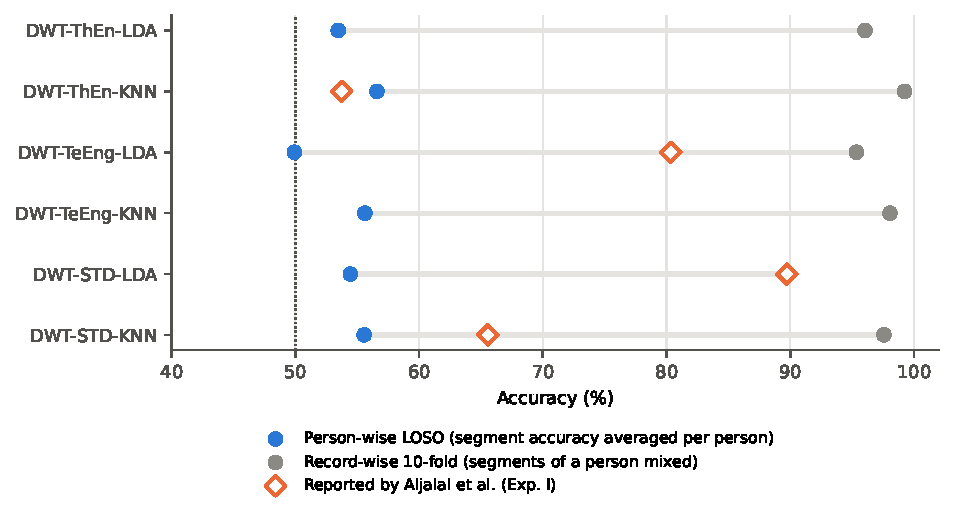
\includegraphics[width=\linewidth]{../figs/en_dev.pdf}
\caption{\textbf{Person-wise versus record-wise validation in the development data.} Same DWT features and classifiers, 19 channels, EEG\_1 (24 people). Blue: LOSO with all segments of the held-out person excluded from training. Grey: 10-fold cross-validation over segments, which mixes segments of the same person. Diamonds: all-channel values reported by \citet{aljalal2024} (Experiment I), where available. Dotted line: 50\%.}
\label{fig:dev}
\end{figure}

\paragraph{Electrode selection fits noise.} Running NSGA-II with shuffled diagnostic labels produced internal LOSO accuracies of 72--79\%, equal to or higher than those obtained with the real labels (65--75\%). In nested LOSO (DWT-ThEn-KNN), the subset chosen on 23 people reached 67\% internally but 40\% on the held-out person. With the cleaner features, the paper's selection rule obtained 48\% in nested LOSO against 61\% without selection, and with shuffled labels one method still reached 71\% under nested evaluation, which illustrates how wide the chance distribution is with 24 people.

\paragraph{Frontal electrodes carry ocular signal.} The share of variance explained by ocular ICA components was 72\% at Fp2, 68\% at Fp1, 52\% at F7 and 39\% at F8, with a clear drop for the remaining electrodes. Horizontal eye-movement activity was larger in the MCI group (uncorrected $p=0.015$; exploratory). Two of the four electrodes most often selected by \citet{aljalal2024} (Fp1 and F8) are therefore among the most contaminated.

\paragraph{Cleaner features did not produce a reliable signal.} ICA cleaning improved balanced accuracy by about 9 points across feature types (from about 48\% to 57\%; $p\approx0.14$). In nested LOSO, M0 reached 61.2\% (AUC 0.61) and M4 64.3\% (AUC 0.61), neither above chance (permutation $p=0.24$ and $0.11$). The leave-pair-out AUC of M0 was 0.65. With the physical montage M0 kept its balanced accuracy (61.2\%; AUC 0.57; leave-pair-out AUC 0.57), but M4 fell to 36.7\% (AUC 0.29) and chose a different combination in almost every fold. These results were known before the preregistration and are why H4 made no prediction for M4-physical.

\subsection{Preregistered external test (EEG\_2)}

The test was run once, after the registration was submitted, with code and feature files whose SHA-256 fingerprints matched the registered ones. Table~\ref{tab:ext} and Fig.~\ref{fig:main} give the results.

\begin{table}[t]
\centering\small
\caption{\textbf{Preregistered external test.} Every method was fitted and selected its electrodes on EEG\_1 (24 people) and was evaluated once on EEG\_2 (34 people: 18 MCI, 16 controls). Balanced accuracy with 95\% stratified bootstrap CI; permutation $p$ with Holm correction across the five main methods. AUC is given where the method produces a continuous score.}
\label{tab:ext}
\begin{tabular}{@{}lccccccc@{}}
\toprule
Method & Electrodes & Correct & Sens. (\%) & Spec. (\%) & Balanced acc. (\%) [95\% CI] & $p_\text{Holm}$ & AUC \\
\midrule
R & 5 & 15/34 & 16.7 & 75.0 & 45.8 [31.2, 60.1] & 1.00 & -- \\
M0 & 15 & 18/34 & 100 & 0 & 50.0 [50.0, 50.0] & 1.00 & 0.52 \\
M4 & 4 & 18/34 & 100 & 0 & 50.0 [50.0, 50.0] & 1.00 & 0.47 \\
M1 & 5\textsuperscript{a} & 18/34 & 100 & 0 & 50.0 [50.0, 50.0] & 1.00 & -- \\
M6 & 5\textsuperscript{a} & 18/34 & 100 & 0 & 50.0 [50.0, 50.0] & 1.00 & -- \\
\midrule
M0-physical & 15 & 18/34 & 72.2 & 31.2 & 51.7 [36.8, 67.0] & --\textsuperscript{b} & 0.44 \\
M4-physical & 4 & 15/34 & 50.0 & 37.5 & 43.8 [28.1, 61.1] & --\textsuperscript{b} & 0.40 \\
\bottomrule
\end{tabular}

\smallskip\footnotesize\raggedright \textsuperscript{a}\,Median over five seeds (range 4--5 for M6). \textsuperscript{b}\,Not part of the chance test family; uncorrected permutation $p=0.56$ and $0.86$.
\end{table}

\begin{figure}[t]
\centering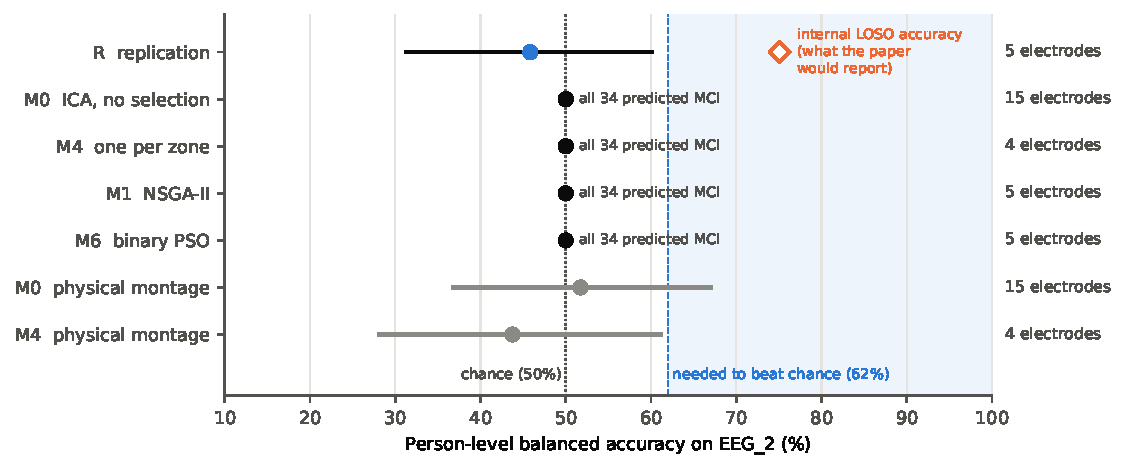
\includegraphics[width=\linewidth]{../figs/en_main.pdf}
\caption{\textbf{No method detected MCI above chance in new people.} Person-level balanced accuracy on EEG\_2 with 95\% bootstrap CI. The shaded area is the range a method needed to reach to beat chance with 34 people. The diamond is the internal LOSO accuracy of the replication on EEG\_1, the figure the original paper's procedure would report. Four methods predicted MCI for all 34 people, so their accuracy is exactly 50\% with no spread.}
\label{fig:main}
\end{figure}

\paragraph{RQ: no method beat chance.} After Holm correction no method performed above chance ($p_\text{Holm}=1.00$ for all five). The replication R classified 15 of 34 people correctly (balanced accuracy 45.8\%), with sensitivity 16.7\% and specificity 75.0\%; its segment-level accuracy was 45.6\%. M0, M4, M1 and M6 predicted MCI for every EEG\_2 person (sensitivity 100\%, specificity 0\%), a degenerate outcome explained in Section~\ref{sec:shift}.

\paragraph{H1 was supported.} On EEG\_1, NSGA-II selected T3, Cz, T4, Pz and P4 (two of them, Cz and T4, among the electrodes most often chosen by \citealp{aljalal2024}) with an internal LOSO accuracy of 75.1\%, the figure the original procedure would report. This value lies above the upper limit of the 95\% CI of the external balanced accuracy (60.1\%); the drop was 29.3 points.

\paragraph{H2 and H3 were met only trivially.} M0 was formally non-inferior to R (difference $+4.2$ points, 90\% CI $-7.6$ to $+16.0$, $p=0.026$), and M4 was formally non-inferior to M1 with fewer electrodes (4 against 5; difference 0, $p_\text{Holm}<0.001$). M6 used the same median number of electrodes as M1, so its part of H3 was not supported. Because M0, M4, M1 and M6 all predicted the same class for every person, these comparisons are uninformative: they show that a constant prediction is not worse than R or than another constant prediction, not that the cleaner or more parsimonious methods detect MCI (Fig.~\ref{fig:diff}).

\paragraph{H4 was inconclusive.} The physical montage changed balanced accuracy by $+1.7$ points for M0 (90\% CI $-10.4$ to $+14.3$; $p_\text{Holm}=0.15$) and by $-6.2$ points for M4 ($-20.5$ to $+8.3$; $p_\text{Holm}=0.31$). Both intervals include the margin and zero, so non-inferiority was not shown and inferiority was not shown either.

\begin{figure}[t]
\centering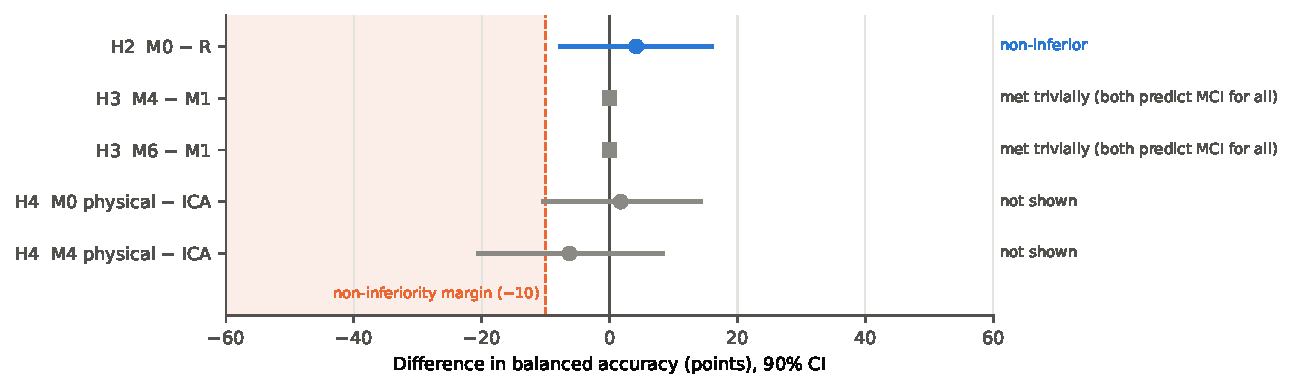
\includegraphics[width=\linewidth]{../figs/en_diff.pdf}
\caption{\textbf{Preregistered paired comparisons.} Difference in balanced accuracy on the same 34 people with 90\% paired bootstrap CI; non-inferiority required the lower limit to be above $-10$ (dashed line). Squares mark comparisons between two methods that predicted MCI for everyone, which are met trivially.}
\label{fig:diff}
\end{figure}

\subsection{Why the methods failed: dataset shift and acquisition confounders}\label{sec:shift}

\paragraph{The two datasets are almost perfectly distinguishable.} The descriptive control classified the dataset of origin of the 58 people from their 15-electrode features with 94.4\% balanced accuracy, far above the 75\% threshold we registered for a large domain shift. In EEG\_2 the delta band accounted for 68.8\% of the 1--30\,Hz power on average, against 39.7\% in EEG\_1, while alpha fell from 21.7\% to 8.0\% (Fig.~\ref{fig:conf}, left). In EEG\_1 the MCI group had more delta than controls (43.5\% against 36.4\%), so every model learned that more delta means MCI; applied to EEG\_2, where everyone has more delta than anyone in EEG\_1, they assigned all 34 people to MCI. Within EEG\_2 the direction was reversed (67.1\% in MCI against 70.7\% in controls).

\begin{figure}[t]
\centering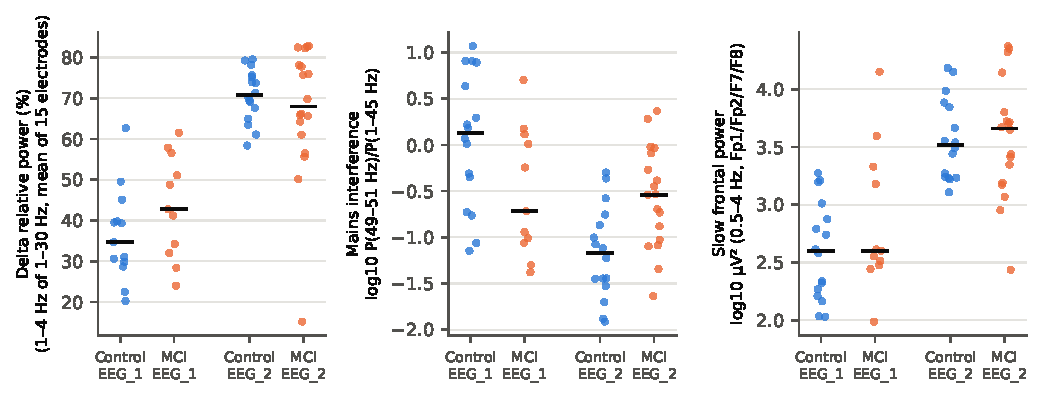
\includegraphics[width=\linewidth]{../figs/en_conf.pdf}
\caption{\textbf{Differences between datasets are larger than differences between groups.} Each dot is a person; bars are medians. Left: delta relative power, the feature that drives the classifiers. Middle: mains interference in the raw recordings; its association with the diagnosis reverses between datasets. Right: slow frontal power, about nine times higher in EEG\_2.}
\label{fig:conf}
\end{figure}

\paragraph{Mains interference is associated with the label, in opposite directions.} The relative power at 49--51\,Hz in the raw recordings differed between datasets ($p<0.001$) and was associated with the diagnosis in both, but in opposite directions: in EEG\_1 controls had more interference than MCI (AUC 0.28 for interference as a predictor of MCI; $p=0.064$), whereas in EEG\_2 MCI had more interference than controls (AUC 0.79; $p=0.004$). Acquisition conditions are thus entangled with the diagnostic groups in a way that does not transfer between datasets.

\paragraph{Model scores track slow frontal activity.} Slow frontal power (0.5--4\,Hz at Fp1, Fp2, F7 and F8) was about nine times higher in EEG\_2 ($p<0.001$) and did not differ between groups within either dataset. In EEG\_2, the continuous score of M0 correlated with this frontal slow power (Spearman $\rho=0.42$, $p=0.012$) and not significantly with the diagnosis (AUC 0.52), even though the frontal electrodes had been removed and ocular components subtracted.

\subsection{Exploratory analyses}

\paragraph{No ranking signal either.} The AUC, which does not depend on the decision threshold and is therefore insensitive to a global shift, was 0.52 for M0, 0.47 for M4, 0.44 for M0-physical and 0.40 for M4-physical. Training on all 27 people of EEG\_1 did not change the picture (AUC 0.41--0.54). In a post hoc analysis that was not preregistered, standardising each dataset with its own mean and standard deviation (without labels) removed the global shift but did not reveal a signal: AUC 0.52 for M0 ($p=0.44$) and 0.45 for M4 with ICA, 0.42 and 0.38 with the physical montage.

\paragraph{The positive control pointed in the expected direction but was weak.} Posterior alpha relative power was lower in MCI than in controls in both datasets, as expected \citep{babiloni2015}, but the effect was small and not significant (AUC 0.59, $p=0.49$ in EEG\_1; 0.57, $p=0.48$ in EEG\_2; similar with the physical montage).

\paragraph{Selected electrodes were stable but not valid.} M1 chose the same subset (F4, T4, T5, Pz, T6) with four of five seeds, and M6 chose T4 and T6 with all five seeds and F4 and Pz with four (Fig.~\ref{fig:heads}). This stability across seeds did not translate into external performance.

\begin{figure}[t]
\centering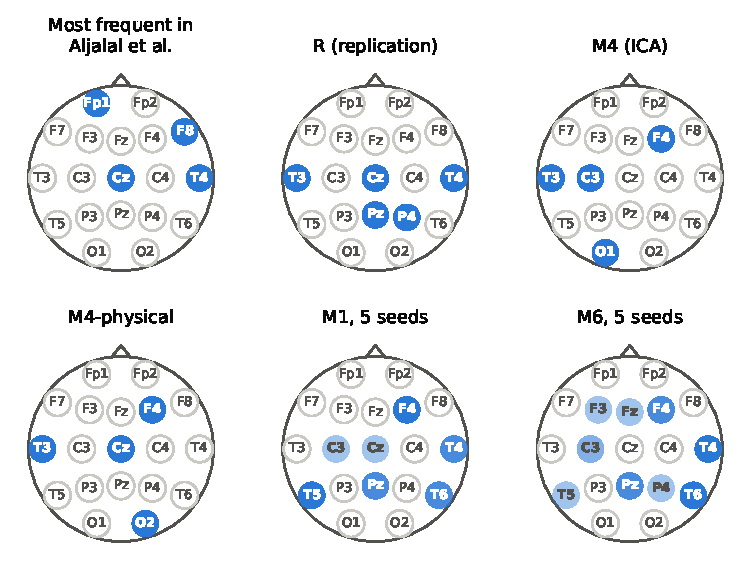
\includegraphics[width=0.82\linewidth]{../figs/en_heads.pdf}
\caption{\textbf{Electrodes selected on EEG\_1.} Darker means selected more often (across seeds for M1 and M6). Fp1 and F8, two of the electrodes most often selected by \citet{aljalal2024}, are among the most contaminated by eye movements; M0--M6 exclude Fp1, Fp2, F7 and F8 by design.}
\label{fig:heads}
\end{figure}

\section{Discussion}

In a preregistered external test, an independent replication of NSGA-II electrode selection for MCI detection reached 75.1\% internal accuracy with five electrodes and 45.8\% balanced accuracy in 34 people it had never seen. Four alternatives built to avoid the known pitfalls did not do better: all of them classified every new person as MCI. No method, with any number of electrodes and with either montage, detected MCI above chance in the new cohort.

\paragraph{Where the published accuracies come from.} Three mechanisms, each measured in the development data, can account for the gap between the published accuracies and our results. First, when segments of the same person are used for training and testing, accuracies of 90--99\% are reached with features that give chance-level results when people are kept separate; the all-channel figure reported by \citet{aljalal2024} is closer to the former. We cannot tell from the paper how the folds were built, so this is a compatibility statement, not a claim about their code. Second, NSGA-II reaches 72--79\% internal accuracy with shuffled labels, so an internal accuracy of 75\% after selection carries no evidence of diagnostic value; nested evaluation and external testing remove this bias \citep{varma2006,cawley2010}. Third, two of the most frequently selected electrodes (Fp1 and F8) are dominated by ocular signal. These mechanisms do not require any error in the original analysis: they are the expected behaviour of an unconstrained search evaluated on the same 24 people, which is why we addressed them by design and by testing on new people.

\paragraph{Dataset shift dominates.} The most informative finding was not planned as a hypothesis: two public datasets from the same centre and recording system are 94\% separable from their EEG alone, and the difference (a delta-dominated spectrum in EEG\_2, nine times more slow frontal power and a different mains interference profile) is larger than any difference between MCI and controls. We cannot determine its cause from the released files; vigilance, electrode impedance, filtering or recording period are possible explanations. Its consequence, however, is clear: a model that has learned a small group difference in delta power will move the whole new cohort across its decision boundary. Per-dataset standardisation removed the global shift but revealed no residual signal, so the failure is not only a calibration problem. The opposite association of mains interference with the diagnosis in the two datasets shows that acquisition conditions can be confounded with the groups. In such small datasets any method that searches widely, whether it optimises electrodes, features or classifiers, is likely to find these confounders.

\paragraph{What the cleaner methods did and did not achieve.} The alternatives were designed to remove three sources of optimism: segment leakage, selection bias and ocular contamination. They succeeded in the sense that their internal estimates were honest (around 61--64\% in nested LOSO, never above chance), but they did not create a signal that does not exist in these data. The formal confirmations of H2 and H3 are therefore not evidence that they work; they only show that their failure was no worse than that of the original method. Parsimonious selection was at least not harmful, and the electrodes selected by NSGA-II and PSO were stable across seeds. Stability, however, did not imply validity: a stable subset can be stably fitted to a confounder.

\paragraph{Virtual versus physical electrodes.} Electrode-minimisation studies usually compute each channel after average referencing and ICA over the full montage, and then report the selected channels as if a device could use them alone. The physical montage tests this directly. In development, the one-per-zone method lost most of its accuracy with physical electrodes; externally, the comparison was inconclusive because neither montage worked. We recommend that future studies report both versions.

\paragraph{Recommendations.} Based on these results we suggest the following minimum protocol for studies that select EEG electrodes for diagnosis: evaluate by person, never by segment; keep selection inside the validation loop (nested); compare against the same procedure run on shuffled labels; report AUC as well as accuracy; check whether the selected electrodes are contaminated by eye movements and whether acquisition variables (such as mains interference) differ between groups; report a physical-montage version; test whether datasets can be told apart before pooling or transferring them; and preregister a single external test \citep{nosek2018,collins2024}.

\paragraph{Limitations.} The sample sizes are small, so the external test could only detect large effects (power 0.84 for a true balanced accuracy of 70\%) and the non-confirmed hypotheses are inconclusive rather than negative. EEG\_2 was released as an extension of the same dataset, but we could not verify that its diagnostic and inclusion criteria, recording protocol or period are identical, and the cause of the dataset shift remains unknown. Our replication rests on documented assumptions where the original paper is not specific (wavelet family, entropy threshold, genetic operators, which controls were excluded), and the external test covered the paper's best channel-selection configuration (DWT, ThEn, discriminant analysis), not every feature combination or the joint feature selection of its Experiment III. Only the first 10 minutes of each recording were analysed, no age or sex information was available, and the ICA component rule was automatic. Some development diagnostics (shuffled labels, ocular contamination) were computed before this registration and are reported as development results. Finally, the per-dataset standardisation was post hoc. None of these limitations favours the conclusion that the original accuracies transfer: each would, if anything, make a transferable signal easier to find.

\section{Conclusions}

The high accuracies reported for NSGA-II electrode selection in MCI detection from resting EEG did not survive an independent, preregistered external test: internal accuracy of 75\% became 46\% in new people, and none of four cleaner or more parsimonious alternatives performed above chance. The decisive factor was a large shift between two datasets from the same centre, together with acquisition variables associated with the diagnostic groups. Minimising electrodes is only meaningful once a signal has been shown to generalise; until then, we recommend person-level, nested and externally validated evaluation, with physical montages and preregistered analyses.
